\documentclass{ieeeaccess}
\usepackage{cite}
\usepackage{amsmath,amssymb,amsfonts}
\usepackage{algorithmic}
\usepackage{graphicx}
\usepackage{textcomp}
\usepackage{booktabs}
\def\BibTeX{{\rm B\kern-.05em{\sc i\kern-.025em b}\kern-.08em
    T\kern-.1667em\lower.7ex\hbox{E}\kern-.125emX}}
\begin{document}
\history{Date of publication xxxx 00, 0000, date of current version xxxx 00, 0000.}
\doi{10.1109/ACCESS.2017.DOI}
\title{Quasi-Newton Methods Comparision using Ackley, Beale, Booth, Matyas, Rastrigin and RosenBrock Functions}
\author{
	\IEEEauthorblockN{Augusto Mathias Adams\IEEEauthorrefmark{1}}
    \IEEEauthorblockN{Caio Phillipe Mizerkowski\IEEEauthorrefmark{2}}
    \IEEEauthorblockN{Christian Piltz Araújo\IEEEauthorrefmark{3}}
    \IEEEauthorblockN{Vinicius Eduardo dos Reis\IEEEauthorrefmark{4}}
	\IEEEauthorblockA{\IEEEauthorrefmark{1}GRR20172143, augusto.adams@ufpr.br}
	\IEEEauthorblockA{\IEEEauthorrefmark{2}GRR20166403, caiomizerkowski@gmail.com}
	\IEEEauthorblockA{\IEEEauthorrefmark{3}GRR20172197, christian0294@yahoo.com.br}
	\IEEEauthorblockA{\IEEEauthorrefmark{4}GRR20175957, eduardo.reis02@gmail.com}
}

\markboth
{Adams \headeretal: Quasi-Newton Methods Comparision using Ackley, Beale, Booth, Matyas, Rastrigin and RosenBrock Functions}
{Adams \headeretal: Quasi-Newton Methods Comparision using Ackley, Beale, Booth, Matyas, Rastrigin and RosenBrock Functions}

\corresp{Corresponding author: Augusto Mathias Adams (e-mail: augusto.adams@ufpr.br).}
\begin{abstract}
This paper discusses briefly four popular algorithms to solve optimization/minimization problems, beloginging to Quasi-Newton class: \textit{Davidon–Fletcher–Powell} (DFP), \textit{Broyden–Fletcher–Goldfarb–Shanno} (BFGS), limited memory BFGS and \textit{Levenberg-Marquardt Algorithm} (LMA). These algorithms are implemented in \textit{Python language}, version 3.10 and uses \textit{SymPy}, \textit{SciPy} and \textit{NumPy} libraries. One of them, \textit{BFGS}, is implemented natively on the  \textit{SciPy} library and the rest are implemented by hand to provide useful insights about the inner operation of the algorithms. The results are, however, very surprising with a few exceptions: when the initial solution is placed in a region near the global minimum, almost all algorithms converges very quickly, so, a study was made to limit the initial solution to  these regions. With exception of 
\end{abstract}

\begin{keywords} 
Optimization Methods, Quasi-Newton, Non-linear Programming
\end{keywords}

\titlepgskip=-15pt

\maketitle

\section{Introduction}
\label{sec:introduction}
\section{2D Function versions}
\label{functions2D}

\subsection{Ackley Function}
\label{ackley2D}

\subsubsection{Convergence Analysis}
\label{convergenceackley2D}

\begin{table}
\centering
\caption{Convergence Report For Ackley Function}
\label{convergence:ackley}
\begin{tabular}{lrrrr}
\toprule
 Alg. &  Good &  Poor &  Diver. &  Total \\
\midrule
  dfp &   100 &     0 &       0 &    100 \\
 bfgs &   100 &     0 &       0 &    100 \\
lbfgs &   100 &     0 &       0 &    100 \\
  lma &   100 &     0 &       0 &    100 \\
\bottomrule
\end{tabular}
\end{table}

\subsubsection{Statistical Analysis of The Solutions}
\label{statisticalanalysisackley2D}

\begin{table}
\centering
\caption{Statistical Information about function values For Ackley Function}
\label{function_values:ackley}
\begin{tabular}{lrrrr}
\toprule
 Alg. &  Min &  Max &  Mean &  Median \\
\midrule
  dfp & 0.00 & 0.00 &  0.00 &    0.00 \\
 bfgs & 0.00 & 0.00 &  0.00 &    0.00 \\
lbfgs & 0.00 & 0.00 &  0.00 &    0.00 \\
  lma & 0.00 & 0.00 &  0.00 &    0.00 \\
\bottomrule
\end{tabular}
\end{table}

\subsubsection{Best Fits}
\label{bestfitsackley2D}

\begin{table}
\centering
\caption{Detailed Solutions For Ackley Function}
\label{solutions:ackley}
\begin{tabular}{llrrr}
\toprule
 Alg. &    Sol. &  Iter. &  F. Eval &  F. Value \\
\midrule
  dfp & $S_{1}$ &     36 &      108 &      0.00 \\
 bfgs & $S_{2}$ &     42 &      129 &      0.00 \\
lbfgs & $S_{3}$ &     37 &      389 &      0.00 \\
  lma & $S_{4}$ &     38 &      320 &      0.00 \\
\bottomrule
\end{tabular}
\end{table}

\subsubsection{Isolines and Convergence line}
\label{isolinesackley2D}

\begin{figure}[h]
                                         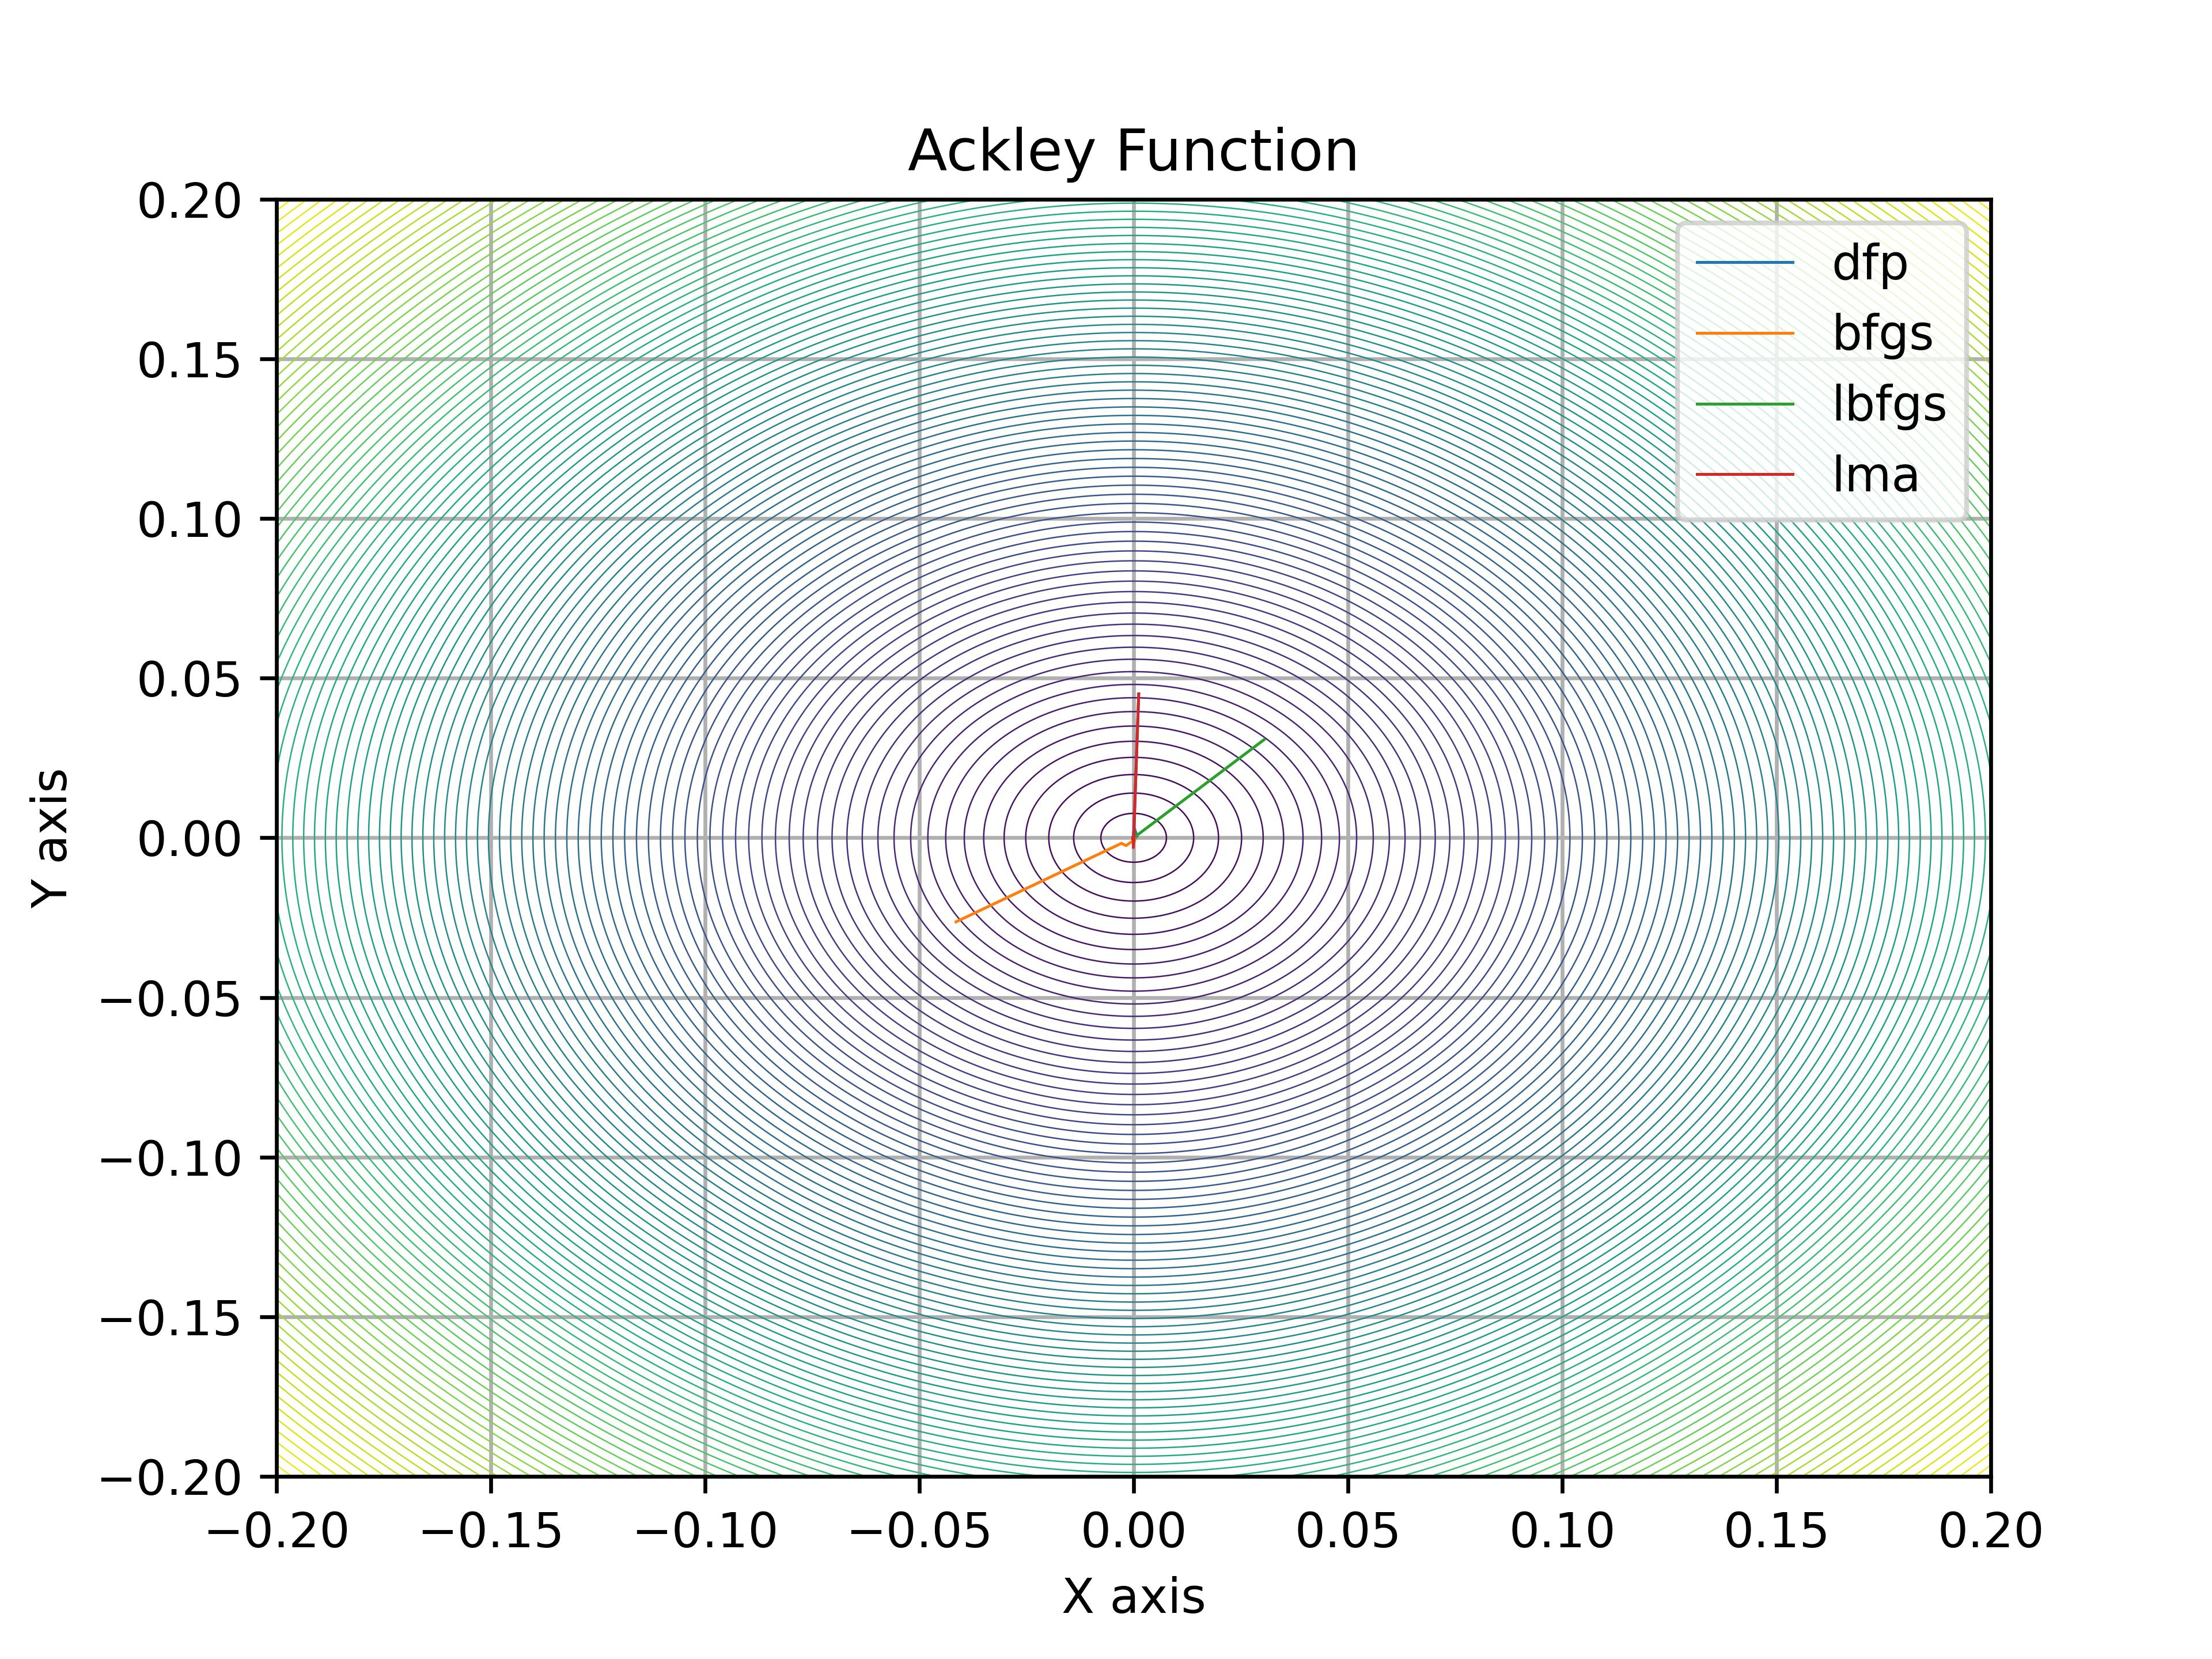
\includegraphics[width=8cm]{images/ackley.jpg}
                                        \end{figure}
                                        
                                        \subsection{Beale Function}
\label{beale2D}

\subsubsection{Convergence Analysis}
\label{convergencebeale2D}

\begin{table}
\centering
\caption{Convergence Report For Beale Function}
\label{convergence:beale}
\begin{tabular}{lrrrr}
\toprule
 Alg. &  Good &  Poor &  Diver. &  Total \\
\midrule
  dfp &    53 &    25 &      22 &    100 \\
 bfgs &    75 &     0 &      25 &    100 \\
lbfgs &    80 &     0 &      20 &    100 \\
  lma &    42 &    37 &      21 &    100 \\
\bottomrule
\end{tabular}
\end{table}

\subsubsection{Statistical Analysis of The Solutions}
\label{statisticalanalysisbeale2D}

\begin{table}
\centering
\caption{Statistical Information about function values For Beale Function}
\label{function_values:beale}
\begin{tabular}{lrrrr}
\toprule
 Alg. &  Min &   Max &  Mean &  Median \\
\midrule
  dfp & 0.00 &  3.84 &  0.27 &    0.00 \\
 bfgs & 0.00 &  0.45 &  0.11 &    0.00 \\
lbfgs & 0.00 &  7.31 &  0.36 &    0.00 \\
  lma & 0.00 & 14.20 &  5.35 &    0.45 \\
\bottomrule
\end{tabular}
\end{table}

\subsubsection{Best Fits}
\label{bestfitsbeale2D}

\begin{table}
\centering
\caption{Detailed Solutions For Beale Function}
\label{solutions:beale}
\begin{tabular}{llrrr}
\toprule
 Alg. &    Sol. &  Iter. &  F. Eval &  F. Value \\
\midrule
  dfp & $S_{1}$ &      8 &       10 &      0.00 \\
 bfgs & $S_{2}$ &     15 &       18 &      0.00 \\
lbfgs & $S_{3}$ &     14 &       50 &      0.00 \\
  lma & $S_{4}$ &     12 &       13 &      0.00 \\
\bottomrule
\end{tabular}
\end{table}

\subsubsection{Isolines and Convergence line}
\label{isolinesbeale2D}

\begin{figure}[h]
                                         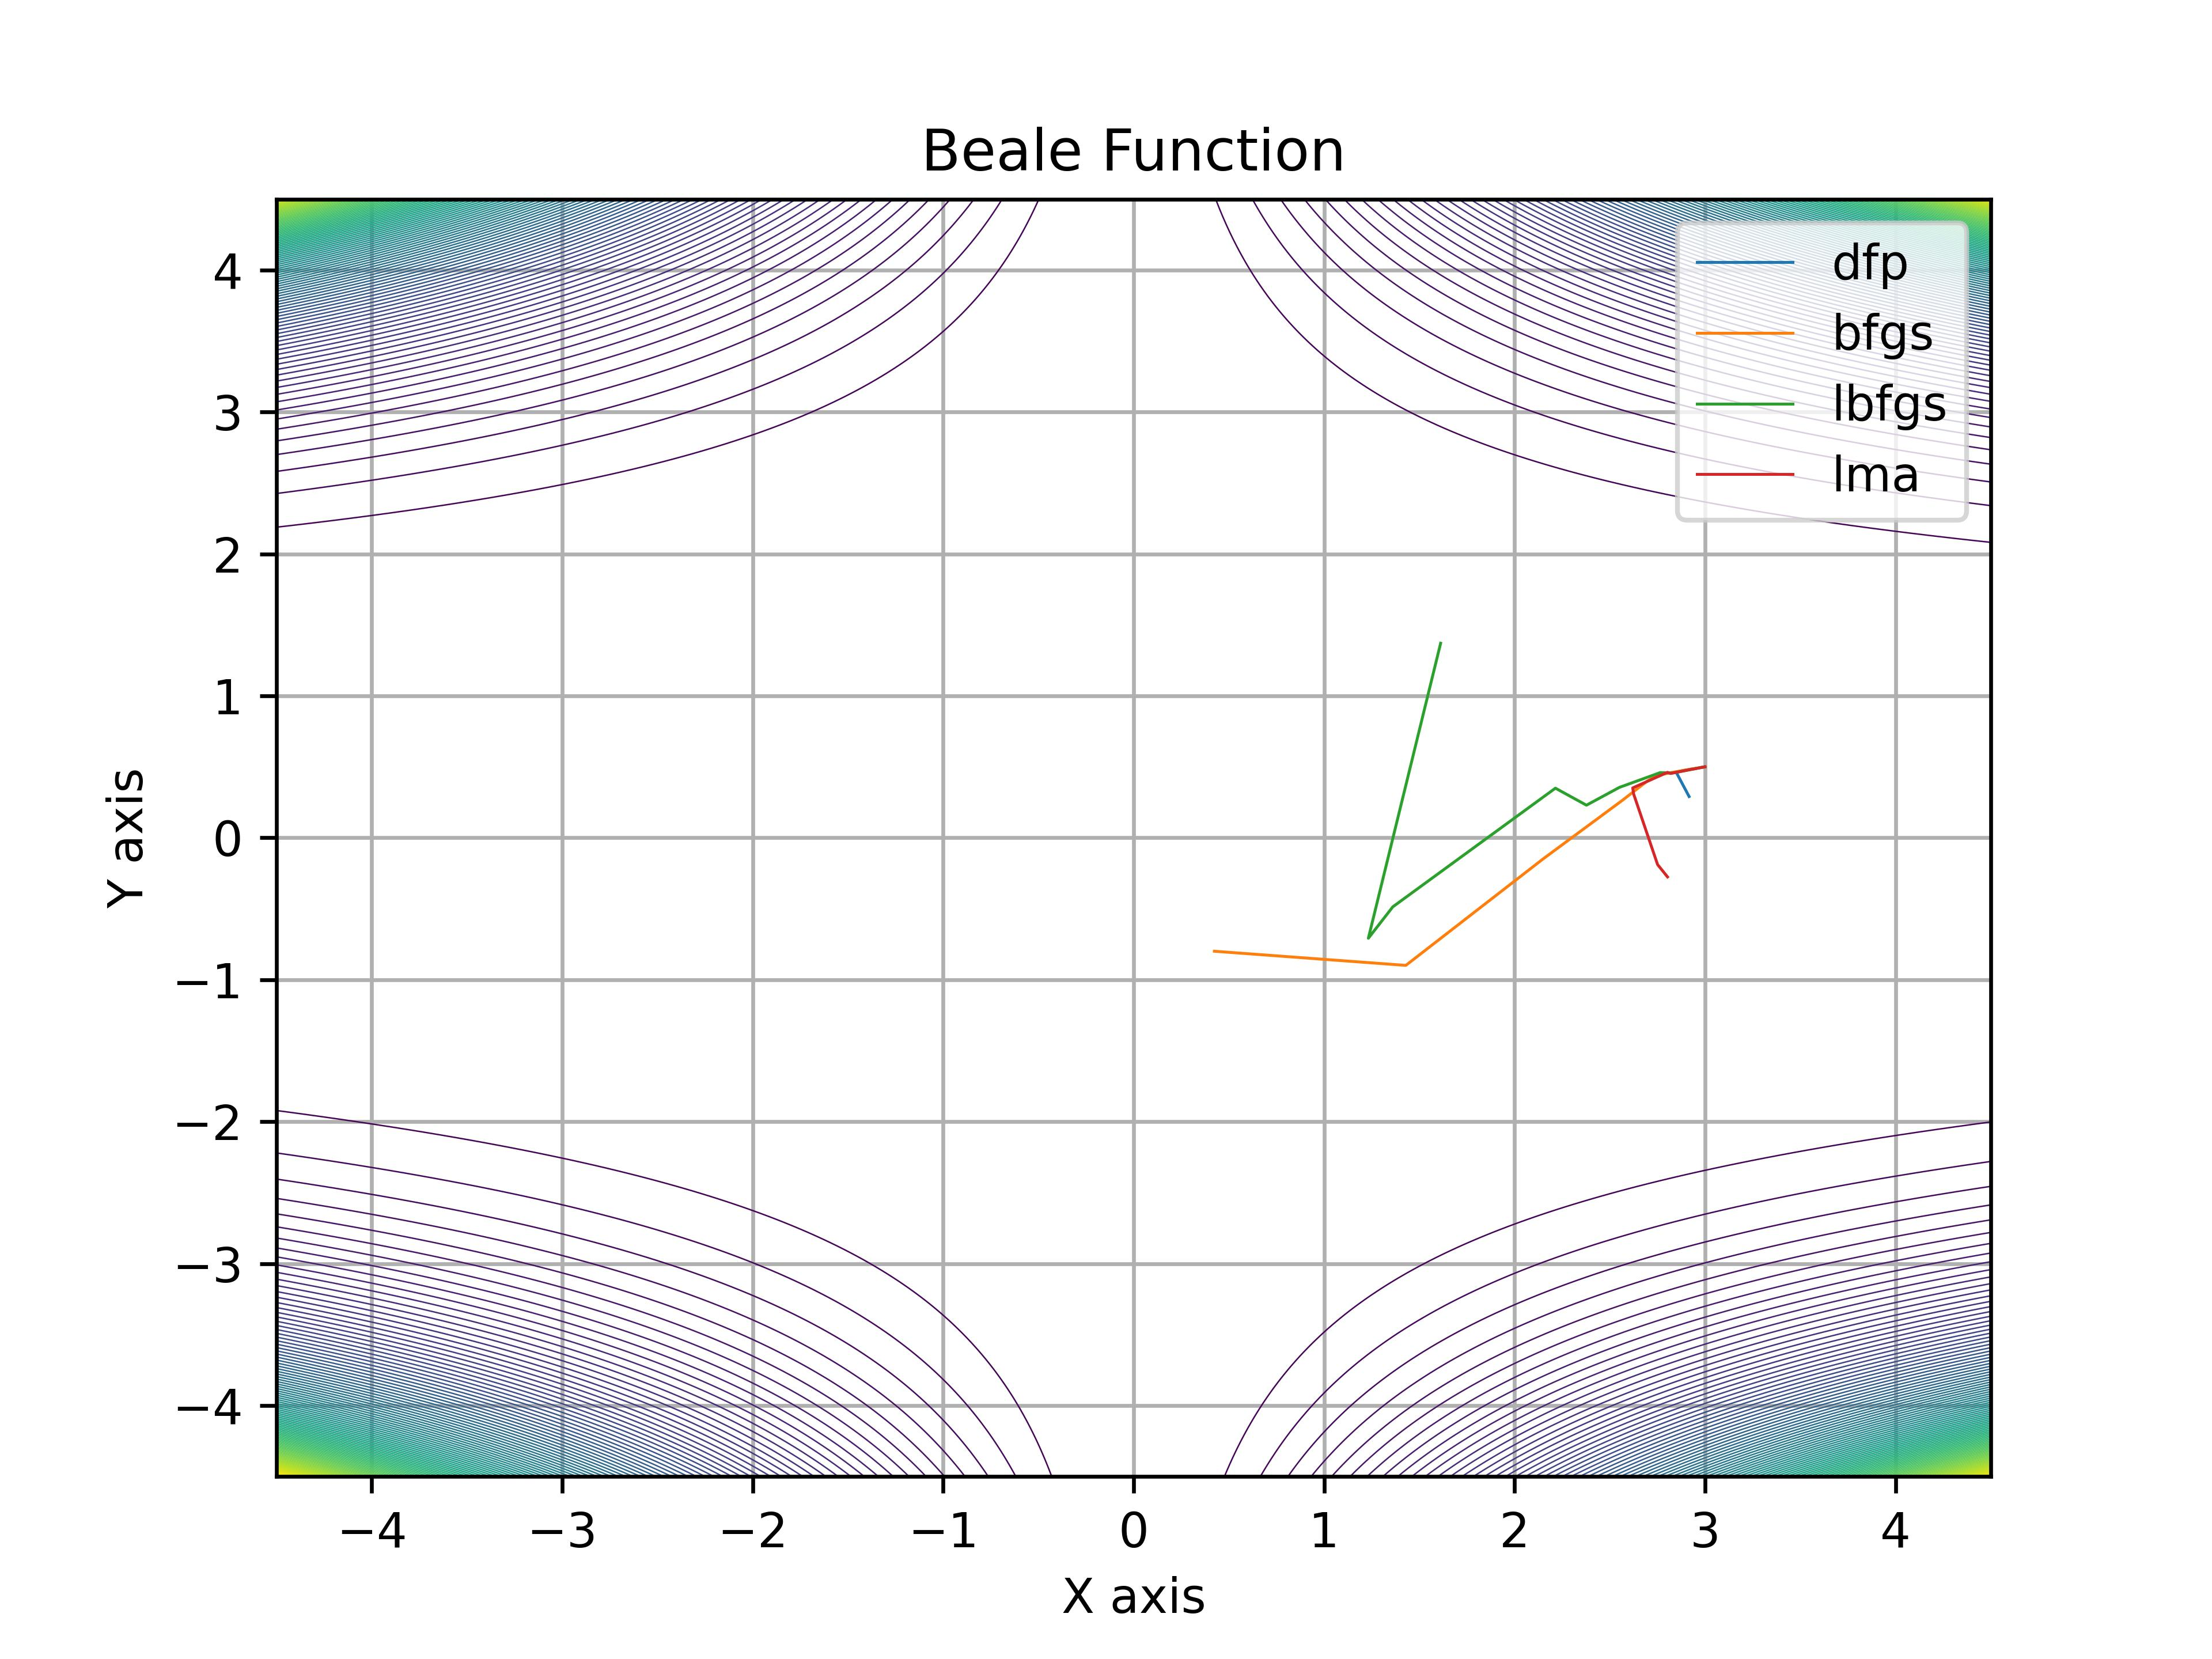
\includegraphics[width=8cm]{images/beale.jpg}
                                        \end{figure}
                                        
                                        \subsection{Booth Function}
\label{booth2D}

\subsubsection{Convergence Analysis}
\label{convergencebooth2D}

\begin{table}
\centering
\caption{Convergence Report For Booth Function}
\label{convergence:booth}
\begin{tabular}{lrrrr}
\toprule
 Alg. &  Good &  Poor &  Diver. &  Total \\
\midrule
  dfp &   100 &     0 &       0 &    100 \\
 bfgs &   100 &     0 &       0 &    100 \\
lbfgs &   100 &     0 &       0 &    100 \\
  lma &   100 &     0 &       0 &    100 \\
\bottomrule
\end{tabular}
\end{table}

\subsubsection{Statistical Analysis of The Solutions}
\label{statisticalanalysisbooth2D}

\begin{table}
\centering
\caption{Statistical Information about function values For Booth Function}
\label{function_values:booth}
\begin{tabular}{lrrrr}
\toprule
 Alg. &  Min &  Max &  Mean &  Median \\
\midrule
  dfp & 0.00 & 0.00 &  0.00 &    0.00 \\
 bfgs & 0.00 & 0.00 &  0.00 &    0.00 \\
lbfgs & 0.00 & 0.00 &  0.00 &    0.00 \\
  lma & 0.00 & 0.00 &  0.00 &    0.00 \\
\bottomrule
\end{tabular}
\end{table}

\subsubsection{Best Fits}
\label{bestfitsbooth2D}

\begin{table}
\centering
\caption{Detailed Solutions For Booth Function}
\label{solutions:booth}
\begin{tabular}{llrrr}
\toprule
 Alg. &    Sol. &  Iter. &  F. Eval &  F. Value \\
\midrule
  dfp & $S_{1}$ &      4 &        6 &      0.00 \\
 bfgs & $S_{2}$ &      2 &        5 &      0.00 \\
lbfgs & $S_{3}$ &      5 &       21 &      0.00 \\
  lma & $S_{4}$ &     10 &       11 &      0.00 \\
\bottomrule
\end{tabular}
\end{table}

\subsubsection{Isolines and Convergence line}
\label{isolinesbooth2D}

\begin{figure}[h]
                                         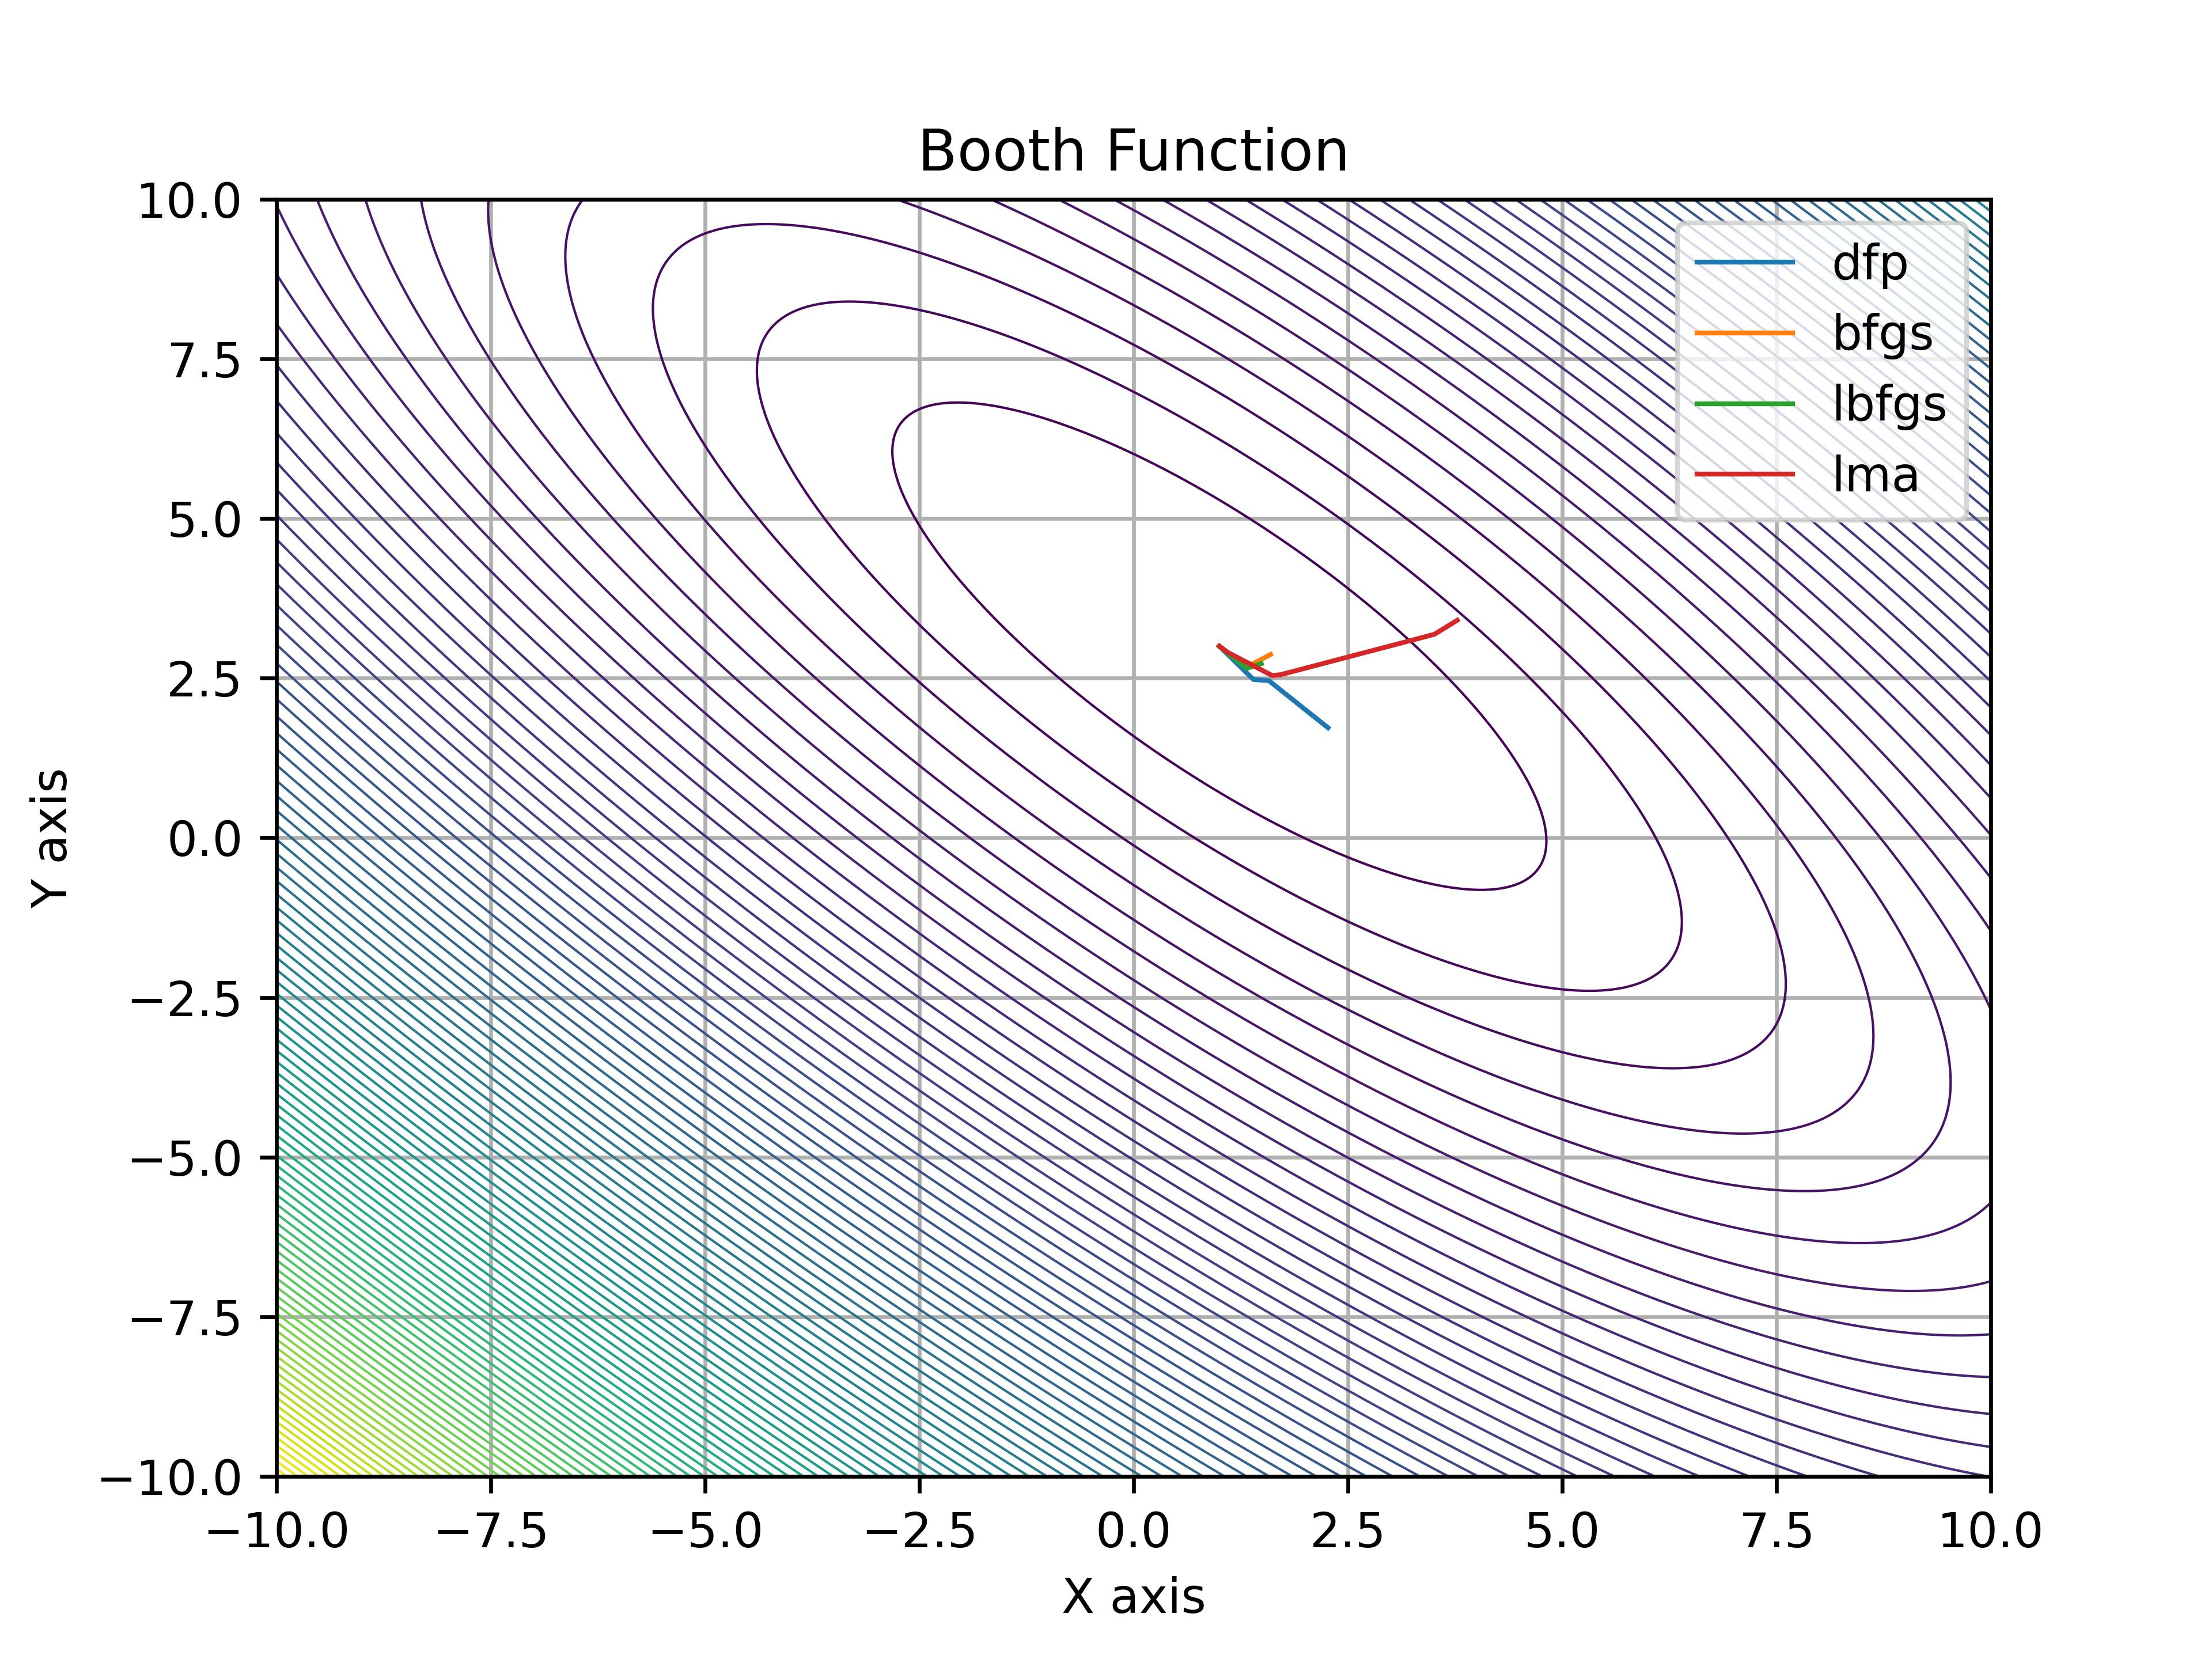
\includegraphics[width=8cm]{images/booth.jpg}
                                        \end{figure}
                                        
                                        \subsection{Matyas Function}
\label{matyas2D}

\subsubsection{Convergence Analysis}
\label{convergencematyas2D}

\begin{table}
\centering
\caption{Convergence Report For Matyas Function}
\label{convergence:matyas}
\begin{tabular}{lrrrr}
\toprule
 Alg. &  Good &  Poor &  Diver. &  Total \\
\midrule
  dfp &   100 &     0 &       0 &    100 \\
 bfgs &   100 &     0 &       0 &    100 \\
lbfgs &   100 &     0 &       0 &    100 \\
  lma &   100 &     0 &       0 &    100 \\
\bottomrule
\end{tabular}
\end{table}

\subsubsection{Statistical Analysis of The Solutions}
\label{statisticalanalysismatyas2D}

\begin{table}
\centering
\caption{Statistical Information about function values For Matyas Function}
\label{function_values:matyas}
\begin{tabular}{lrrrr}
\toprule
 Alg. &  Min &  Max &  Mean &  Median \\
\midrule
  dfp & 0.00 & 0.00 &  0.00 &    0.00 \\
 bfgs & 0.00 & 0.00 &  0.00 &    0.00 \\
lbfgs & 0.00 & 0.00 &  0.00 &    0.00 \\
  lma & 0.00 & 0.00 &  0.00 &    0.00 \\
\bottomrule
\end{tabular}
\end{table}

\subsubsection{Best Fits}
\label{bestfitsmatyas2D}

\begin{table}
\centering
\caption{Detailed Solutions For Matyas Function}
\label{solutions:matyas}
\begin{tabular}{llrrr}
\toprule
 Alg. &    Sol. &  Iter. &  F. Eval &  F. Value \\
\midrule
  dfp & $S_{1}$ &      7 &       10 &      0.00 \\
 bfgs & $S_{2}$ &      7 &       10 &      0.00 \\
lbfgs & $S_{3}$ &      4 &       16 &      0.00 \\
  lma & $S_{4}$ &     14 &       15 &      0.00 \\
\bottomrule
\end{tabular}
\end{table}

\subsubsection{Isolines and Convergence line}
\label{isolinesmatyas2D}

\begin{figure}[h]
                                         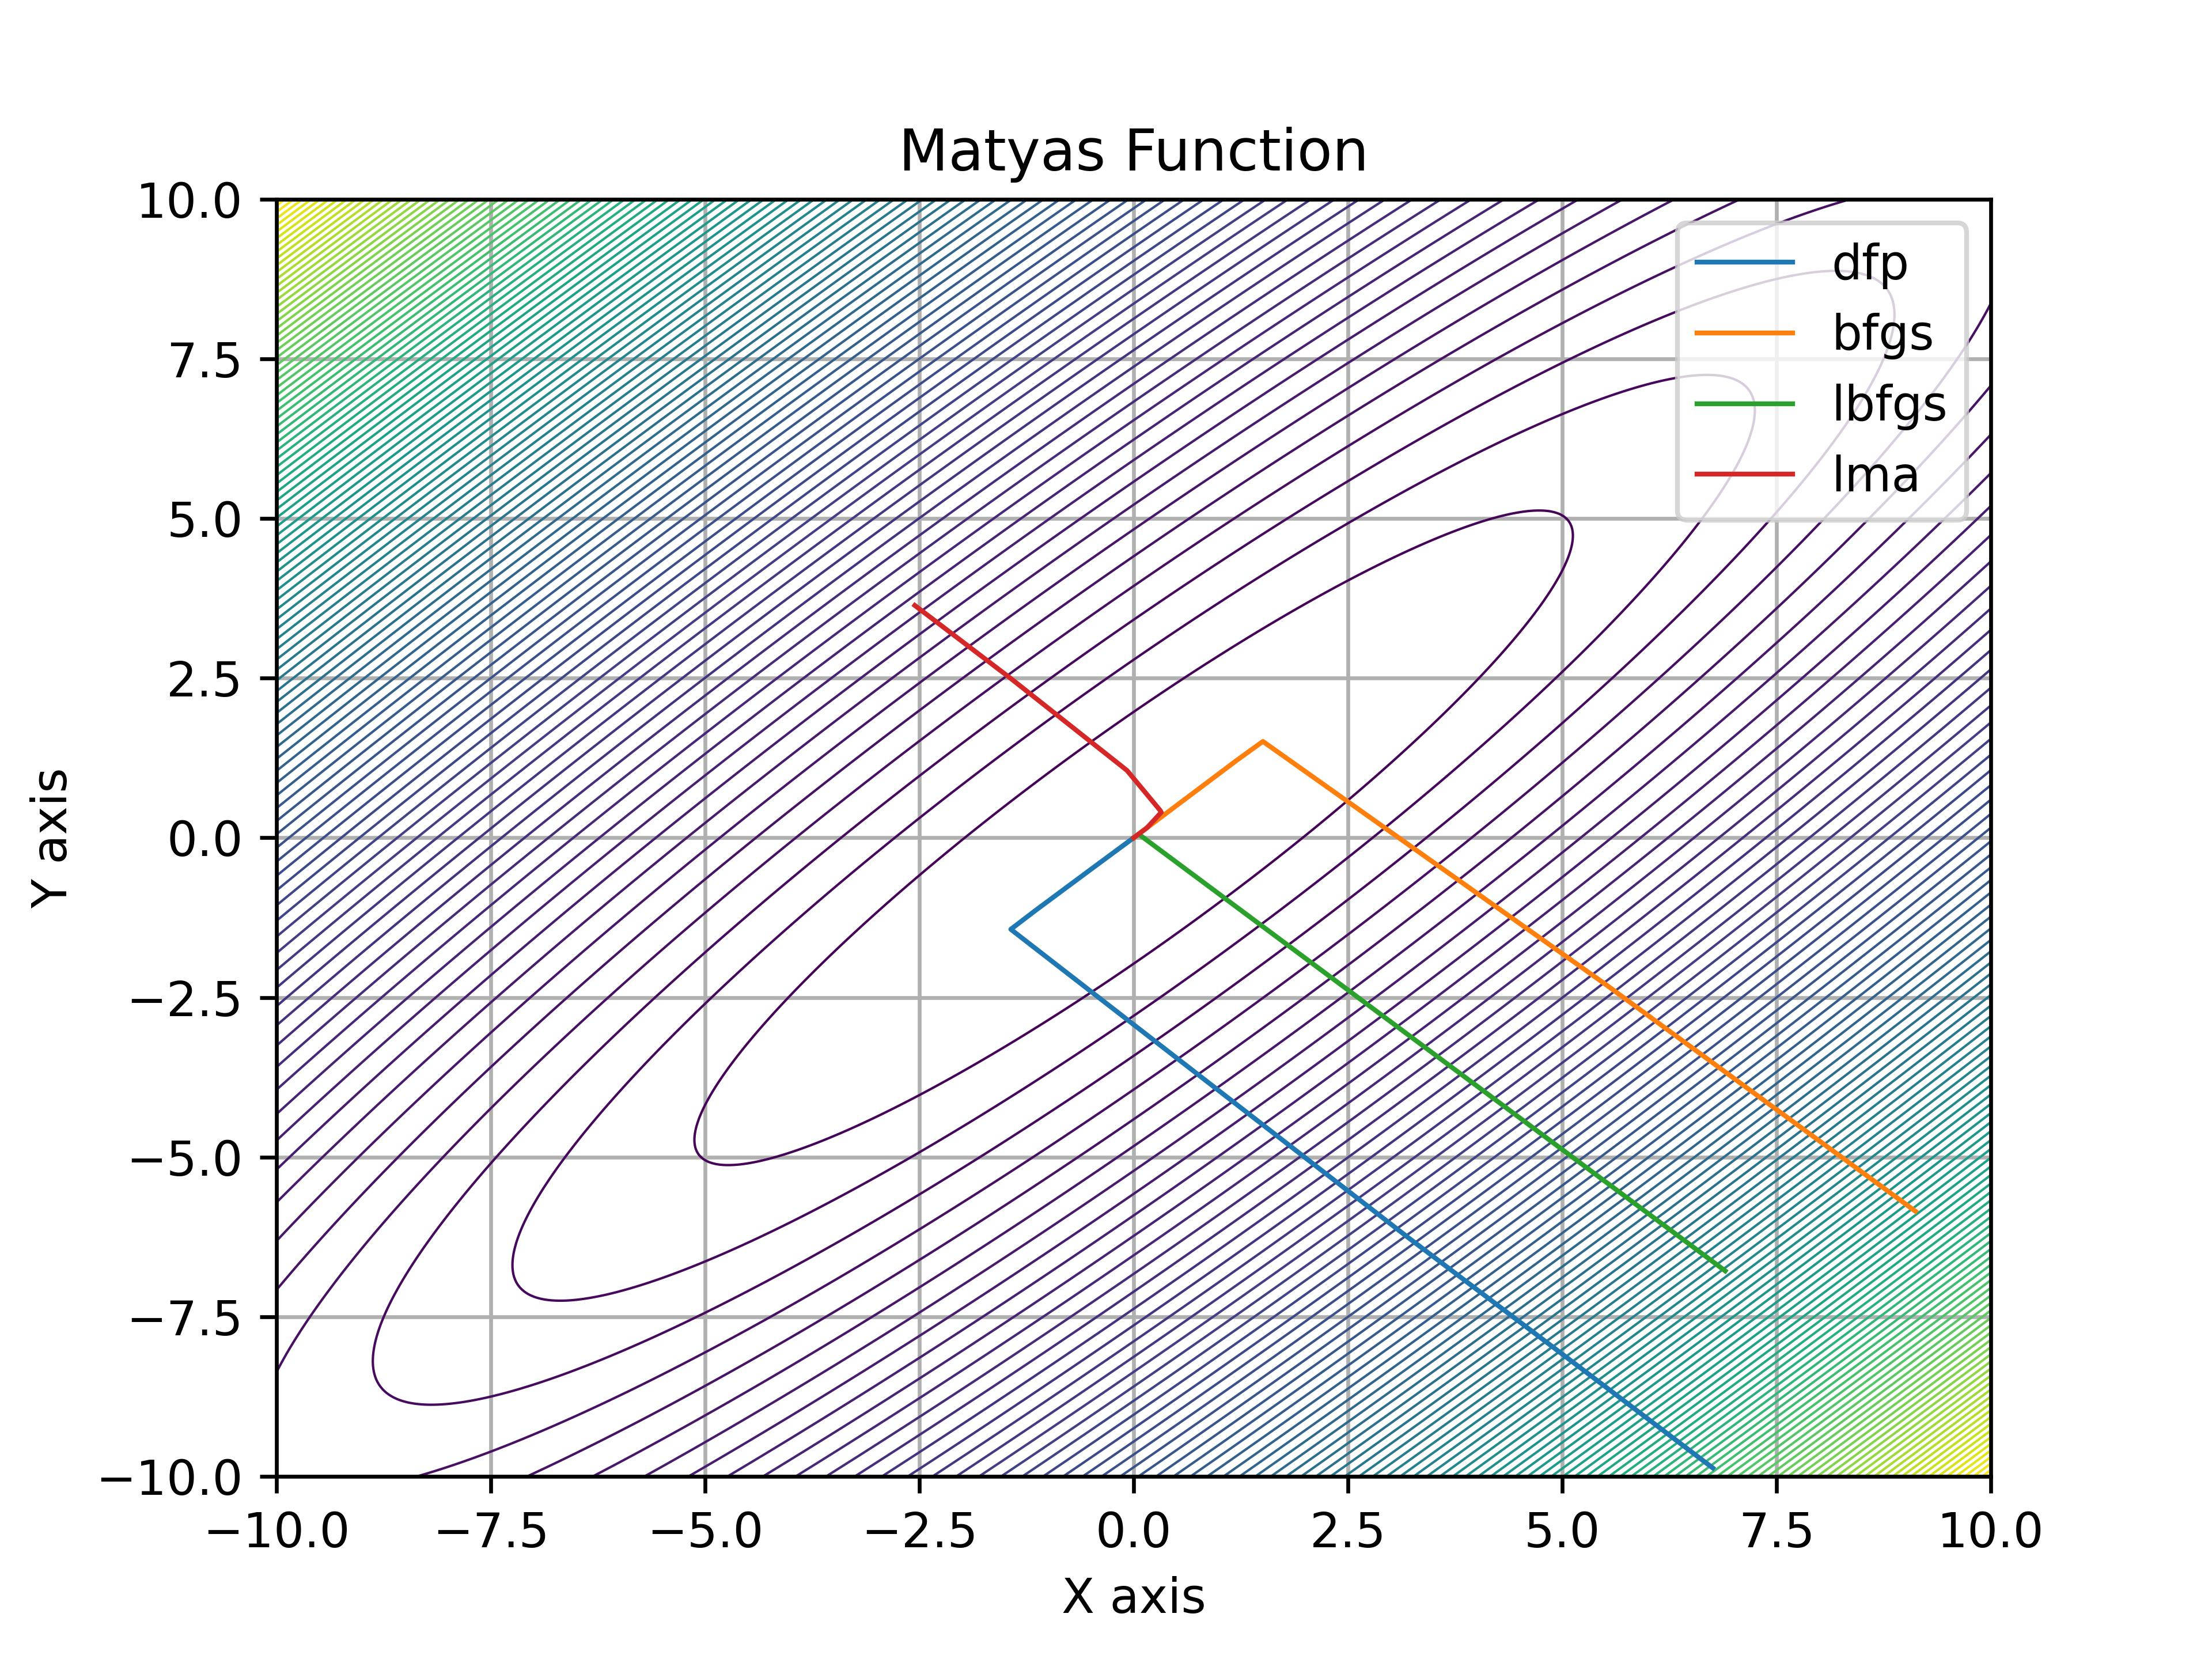
\includegraphics[width=8cm]{images/matyas.jpg}
                                        \end{figure}
                                        
                                        \subsection{Rastrigin Function}
\label{rastrigin2d2D}

\subsubsection{Convergence Analysis}
\label{convergencerastrigin2d2D}

\begin{table}
\centering
\caption{Convergence Report For Rastrigin Function}
\label{convergence:rastrigin2d}
\begin{tabular}{lrrrr}
\toprule
 Alg. &  Good &  Poor &  Diver. &  Total \\
\midrule
  dfp &   100 &     0 &       0 &    100 \\
 bfgs &   100 &     0 &       0 &    100 \\
lbfgs &    99 &     1 &       0 &    100 \\
  lma &   100 &     0 &       0 &    100 \\
\bottomrule
\end{tabular}
\end{table}

\subsubsection{Statistical Analysis of The Solutions}
\label{statisticalanalysisrastrigin2d2D}

\begin{table}
\centering
\caption{Statistical Information about function values For Rastrigin Function}
\label{function_values:rastrigin2d}
\begin{tabular}{lrrrr}
\toprule
 Alg. &  Min &  Max &  Mean &  Median \\
\midrule
  dfp & 0.00 & 0.00 &  0.00 &    0.00 \\
 bfgs & 0.00 & 0.00 &  0.00 &    0.00 \\
lbfgs & 0.00 & 1.99 &  0.02 &    0.00 \\
  lma & 0.00 & 0.00 &  0.00 &    0.00 \\
\bottomrule
\end{tabular}
\end{table}

\subsubsection{Best Fits}
\label{bestfitsrastrigin2d2D}

\begin{table}
\centering
\caption{Detailed Solutions For Rastrigin Function}
\label{solutions:rastrigin2d}
\begin{tabular}{llrrr}
\toprule
 Alg. &    Sol. &  Iter. &  F. Eval &  F. Value \\
\midrule
  dfp & $S_{1}$ &      6 &       11 &      0.00 \\
 bfgs & $S_{2}$ &      8 &       49 &      0.00 \\
lbfgs & $S_{3}$ &      5 &      133 &      0.00 \\
  lma & $S_{4}$ &      4 &        5 &      0.00 \\
\bottomrule
\end{tabular}
\end{table}

\subsubsection{Isolines and Convergence line}
\label{isolinesrastrigin2d2D}

\begin{figure}[h]
                                         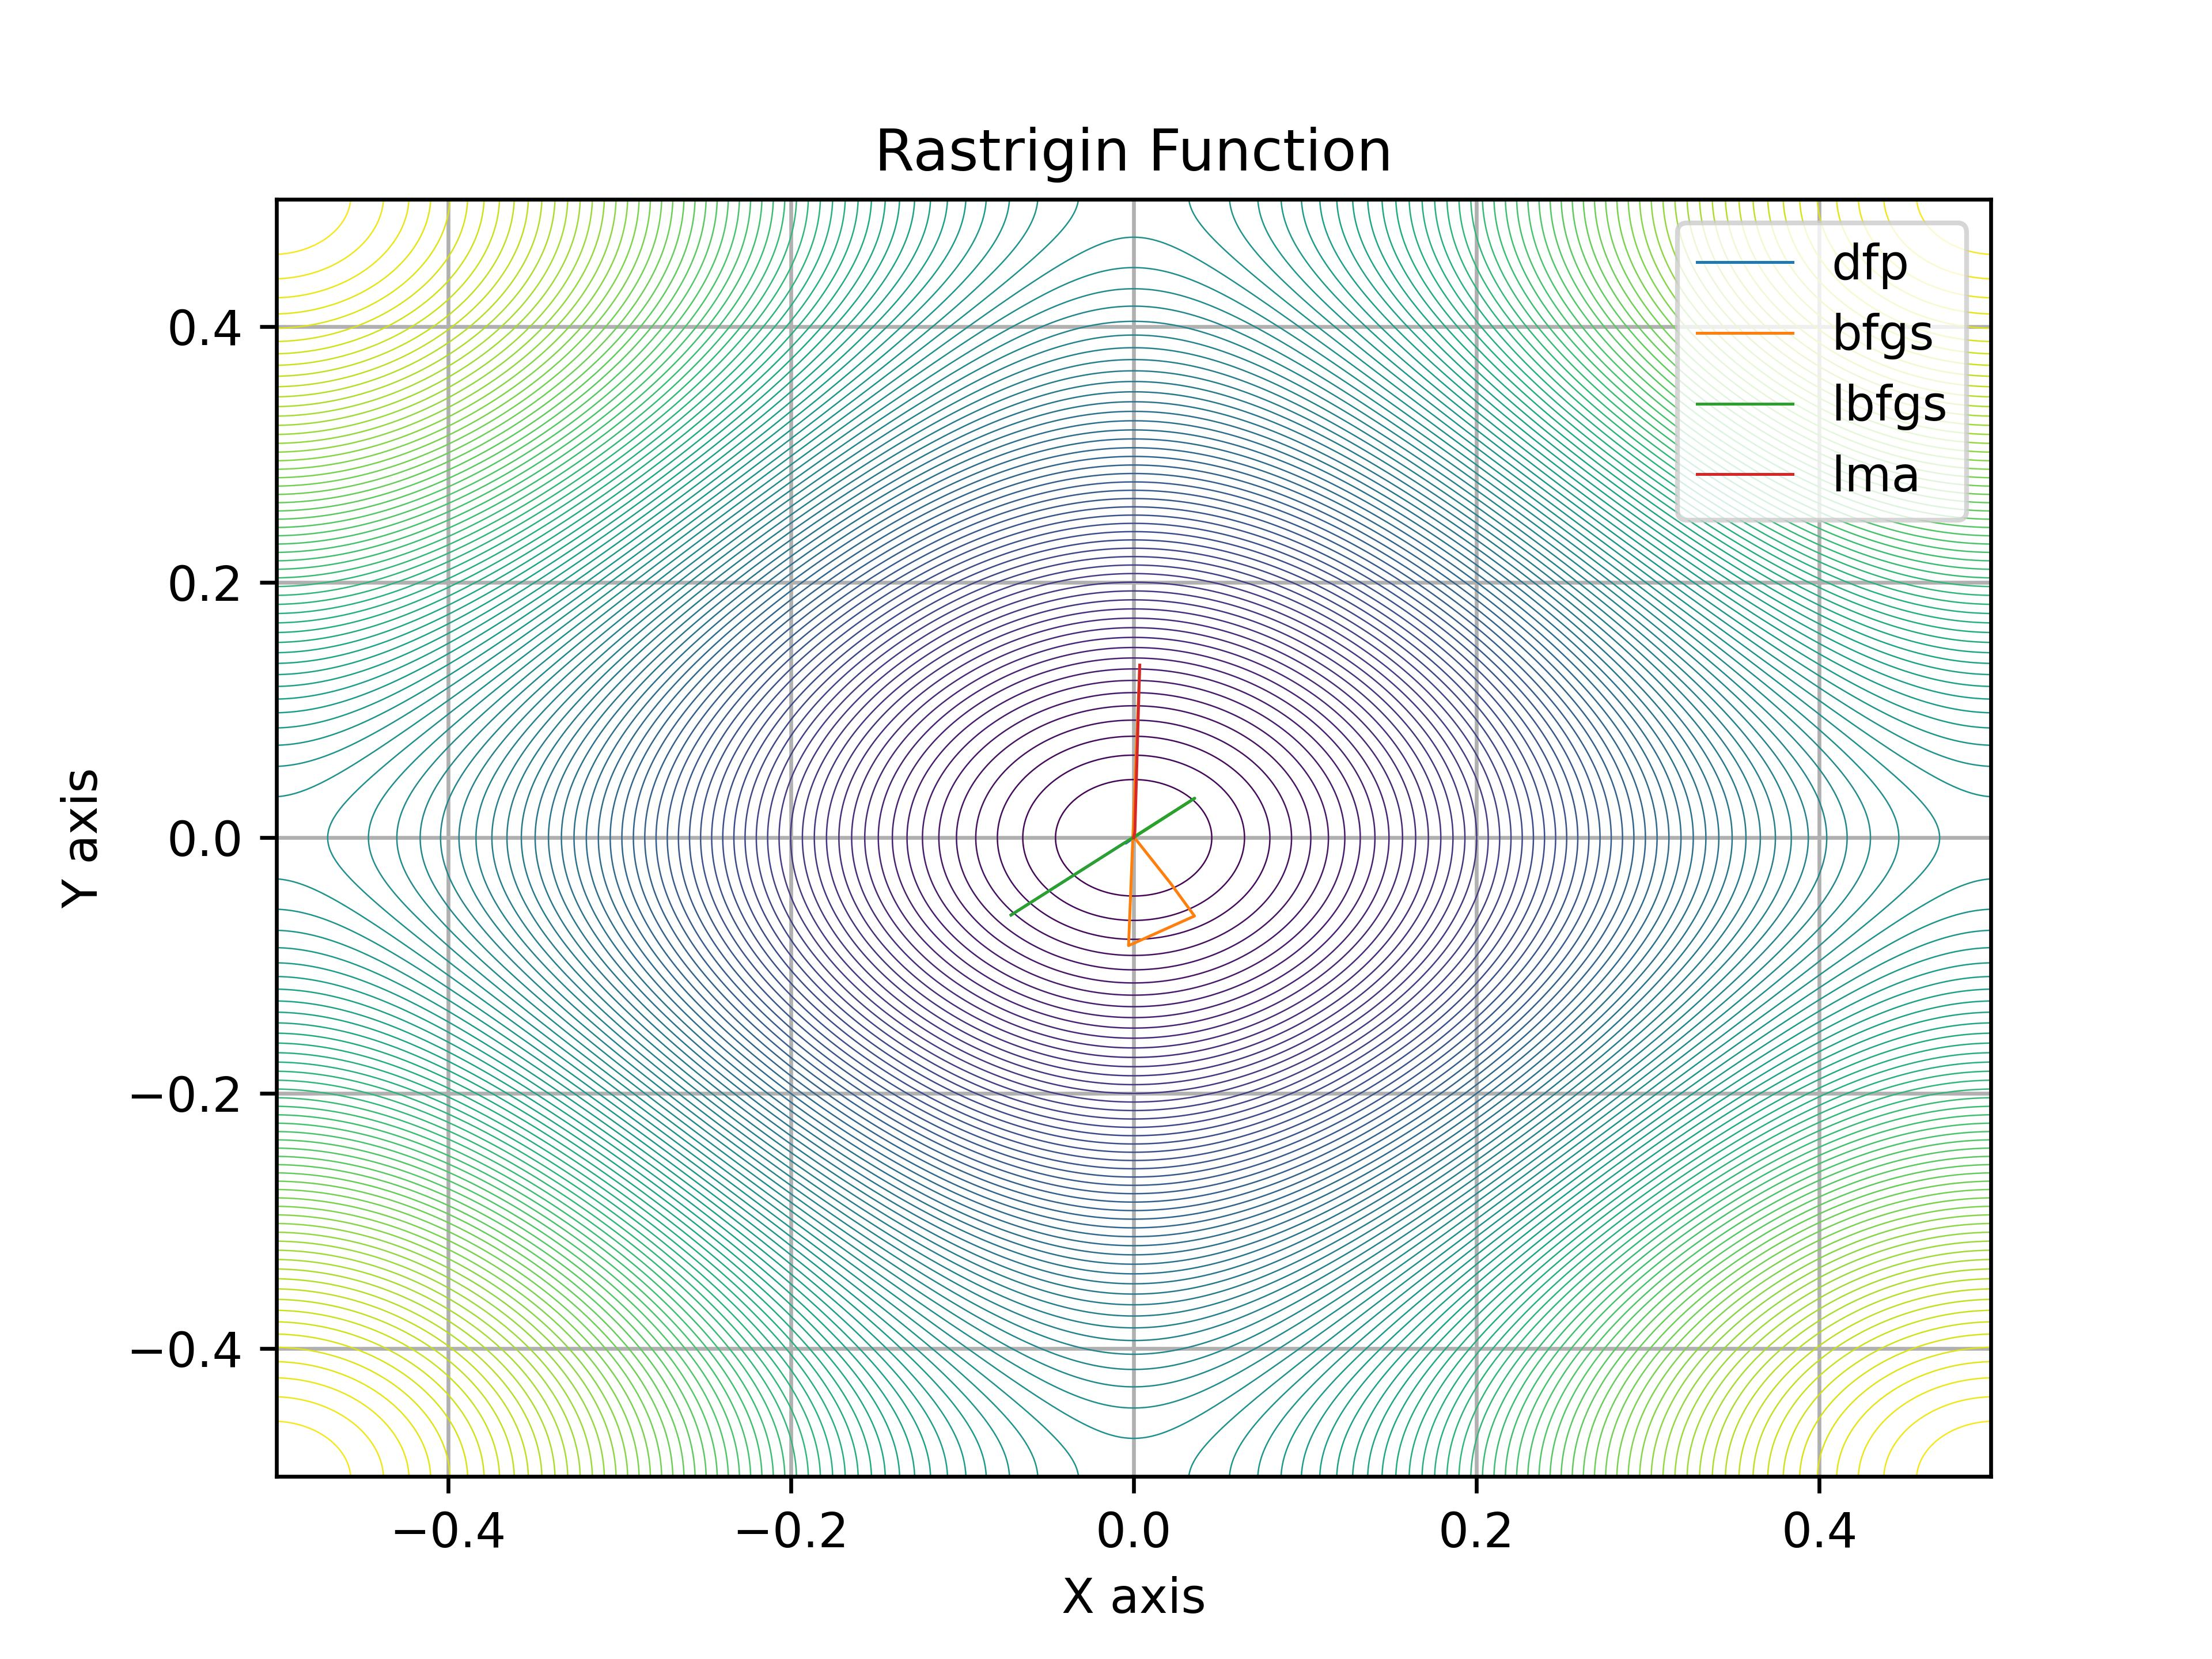
\includegraphics[width=8cm]{images/rastrigin2d.jpg}
                                        \end{figure}
                                        
                                        \subsection{Rosenbrock Function}
\label{rosenbrock2d2D}

\subsubsection{Convergence Analysis}
\label{convergencerosenbrock2d2D}

\begin{table}
\centering
\caption{Convergence Report For Rosenbrock Function}
\label{convergence:rosenbrock2d}
\begin{tabular}{lrrrr}
\toprule
 Alg. &  Good &  Poor &  Diver. &  Total \\
\midrule
  dfp &    74 &    26 &       0 &    100 \\
 bfgs &   100 &     0 &       0 &    100 \\
lbfgs &   100 &     0 &       0 &    100 \\
  lma &   100 &     0 &       0 &    100 \\
\bottomrule
\end{tabular}
\end{table}

\subsubsection{Statistical Analysis of The Solutions}
\label{statisticalanalysisrosenbrock2d2D}

\begin{table}
\centering
\caption{Statistical Information about function values For Rosenbrock Function}
\label{function_values:rosenbrock2d}
\begin{tabular}{lrrrr}
\toprule
 Alg. &  Min &  Max &  Mean &  Median \\
\midrule
  dfp & 0.00 & 1.33 &  0.04 &    0.00 \\
 bfgs & 0.00 & 0.00 &  0.00 &    0.00 \\
lbfgs & 0.00 & 0.00 &  0.00 &    0.00 \\
  lma & 0.00 & 0.00 &  0.00 &    0.00 \\
\bottomrule
\end{tabular}
\end{table}

\subsubsection{Best Fits}
\label{bestfitsrosenbrock2d2D}

\begin{table}
\centering
\caption{Detailed Solutions For Rosenbrock Function}
\label{solutions:rosenbrock2d}
\begin{tabular}{llrrr}
\toprule
 Alg. &    Sol. &  Iter. &  F. Eval &  F. Value \\
\midrule
  dfp & $S_{1}$ &     24 &       31 &      0.00 \\
 bfgs & $S_{2}$ &     30 &       43 &      0.00 \\
lbfgs & $S_{3}$ &     27 &       76 &      0.00 \\
  lma & $S_{4}$ &     16 &       18 &      0.00 \\
\bottomrule
\end{tabular}
\end{table}

\subsubsection{Isolines and Convergence line}
\label{isolinesrosenbrock2d2D}

\begin{figure}[h]
                                         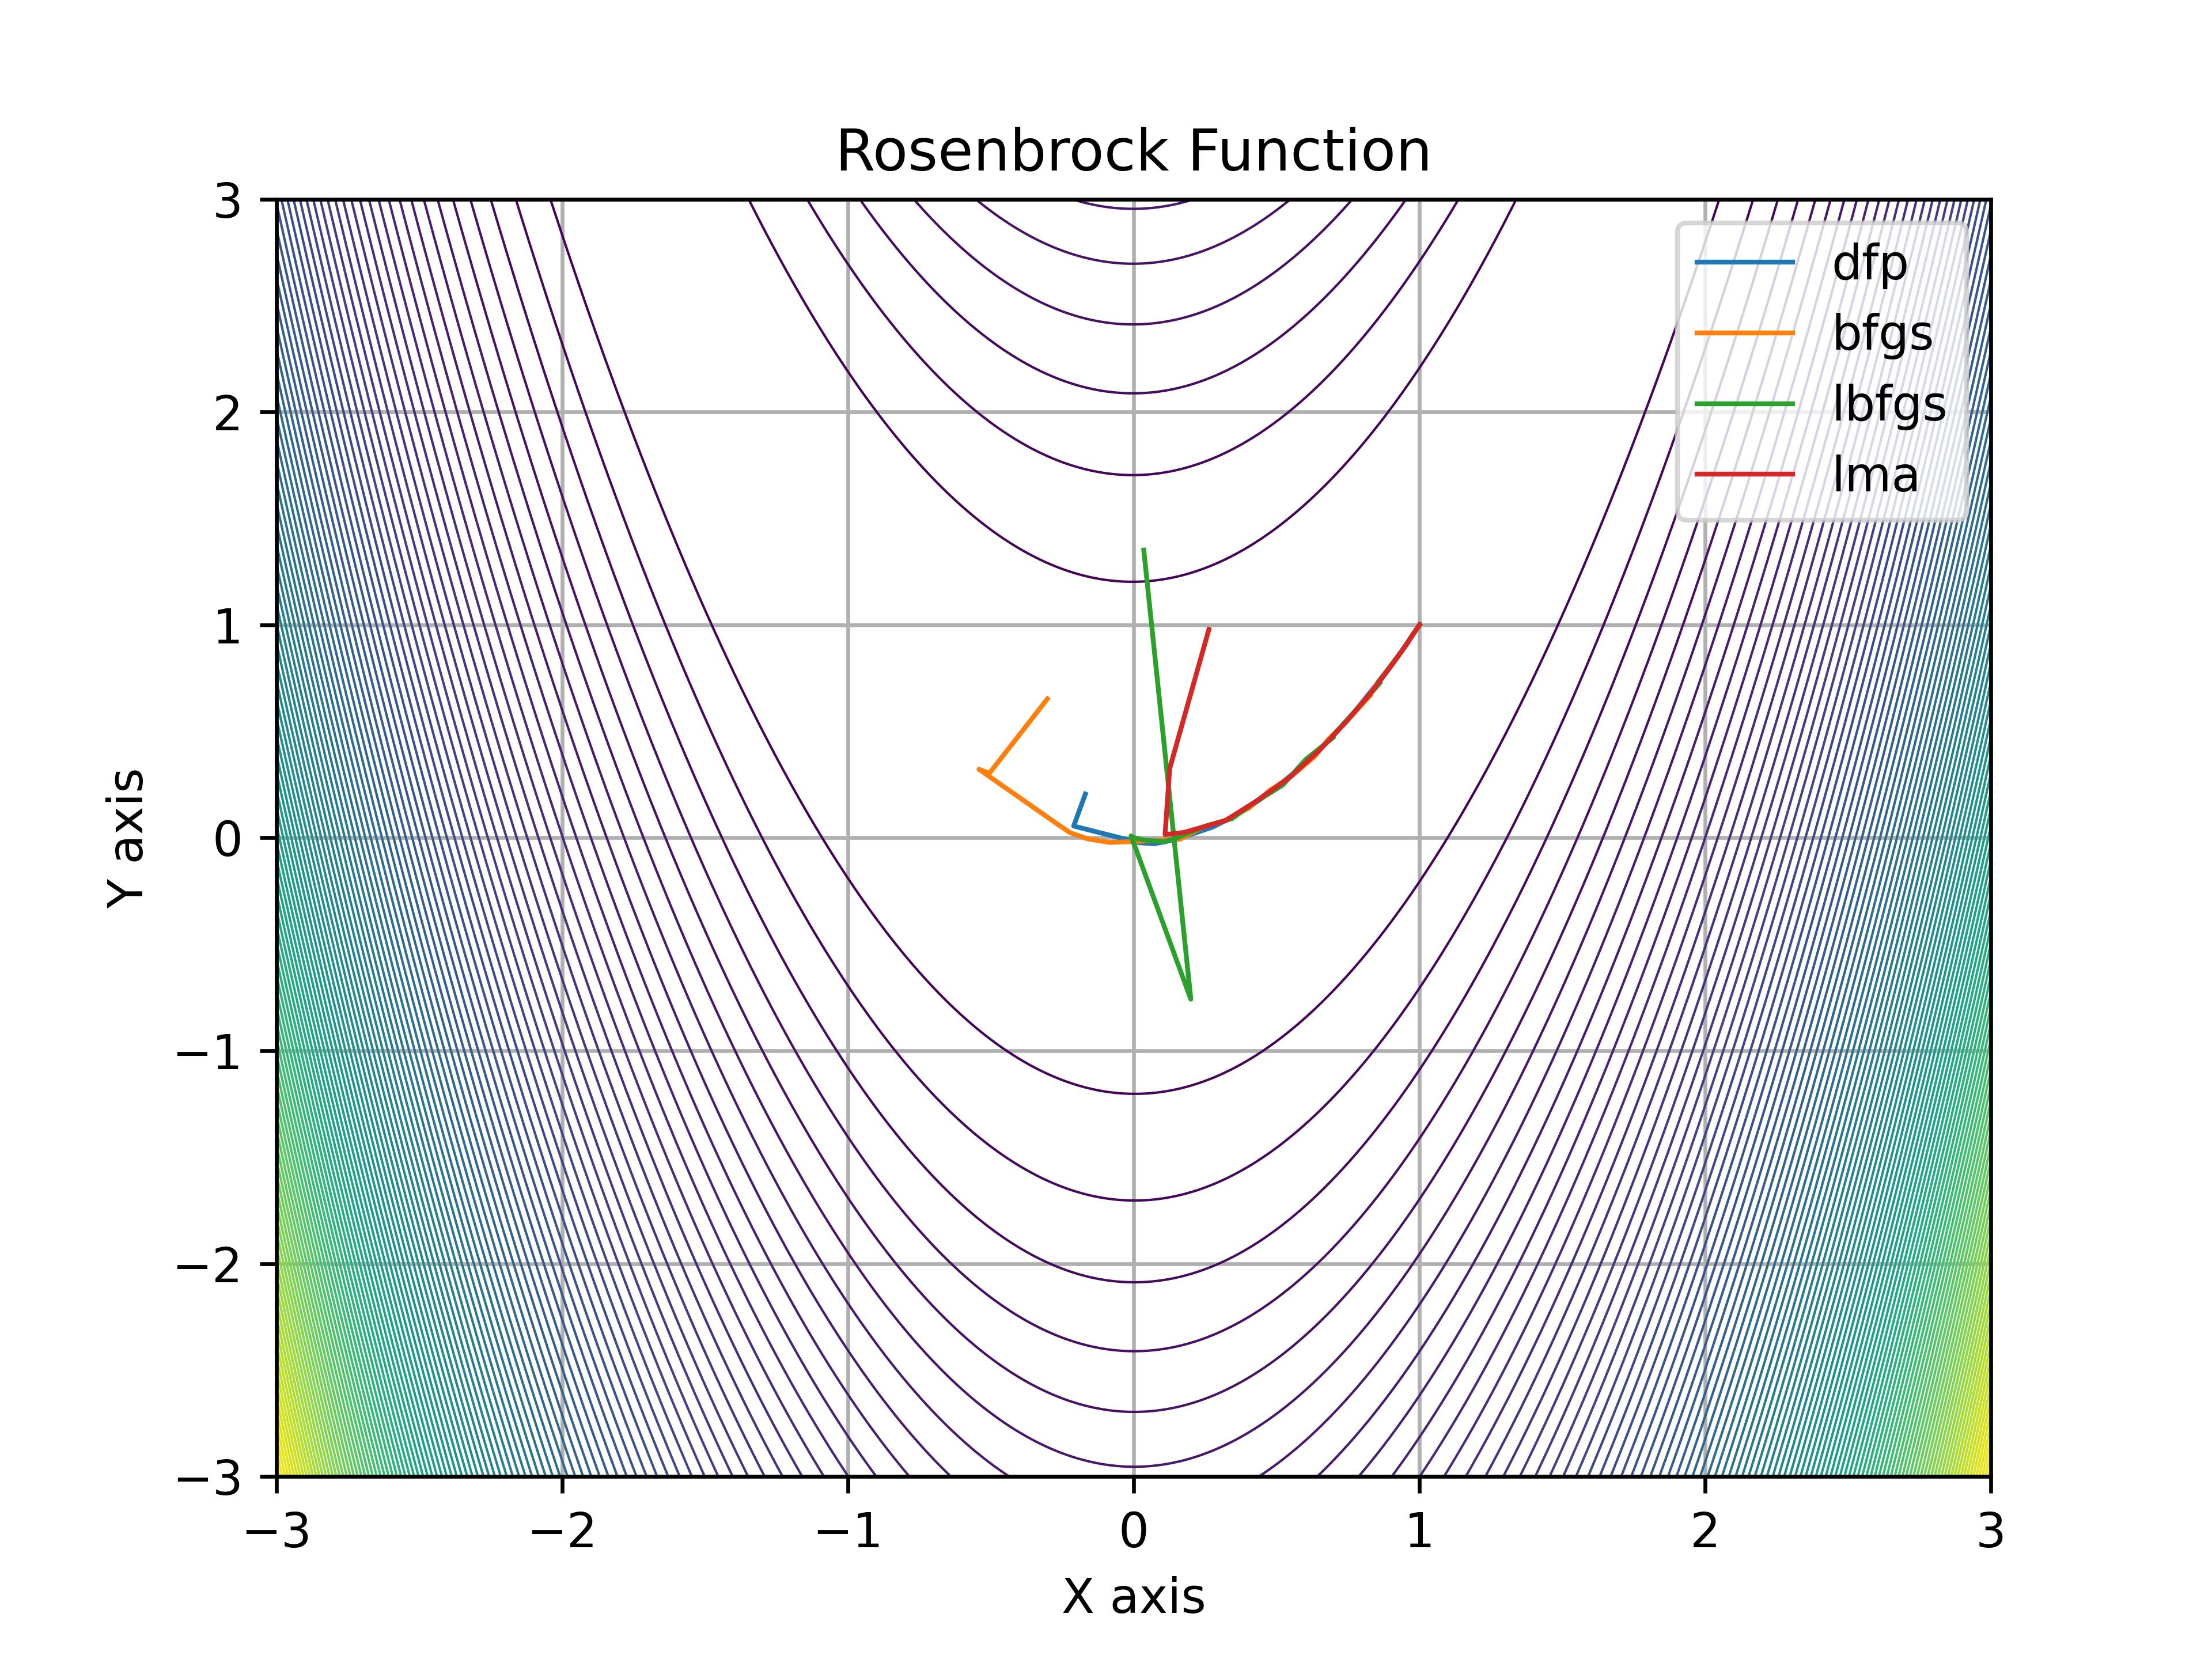
\includegraphics[width=8cm]{images/rosenbrock2d.jpg}
                                        \end{figure}
                                        
                                        
\section{4D Function versions}
\label{functions4D}

\subsection{Rastrigin Function}
\label{rastrigin4d4D}

\subsubsection{Convergence Analysis}
\label{convergencerastrigin4d4D}

\begin{table}
\centering
\caption{Convergence Report For Rastrigin Function}
\label{convergence:rastrigin4d}
\begin{tabular}{lrrrr}
\toprule
 Alg. &  Good &  Poor &  Diver. &  Total \\
\midrule
  dfp &   100 &     0 &       0 &    100 \\
 bfgs &   100 &     0 &       0 &    100 \\
lbfgs &   100 &     0 &       0 &    100 \\
  lma &   100 &     0 &       0 &    100 \\
\bottomrule
\end{tabular}
\end{table}

\subsubsection{Statistical Analysis of The Solutions}
\label{statisticalanalysisrastrigin4d4D}

\begin{table}
\centering
\caption{Statistical Information about function values For Rastrigin Function}
\label{function_values:rastrigin4d}
\begin{tabular}{lrrrr}
\toprule
 Alg. &  Min &  Max &  Mean &  Median \\
\midrule
  dfp & 0.00 & 0.00 &  0.00 &    0.00 \\
 bfgs & 0.00 & 0.00 &  0.00 &    0.00 \\
lbfgs & 0.00 & 0.00 &  0.00 &    0.00 \\
  lma & 0.00 & 0.00 &  0.00 &    0.00 \\
\bottomrule
\end{tabular}
\end{table}

\subsubsection{Best Fits}
\label{bestfitsrastrigin4d4D}

\begin{table}
\centering
\caption{Detailed Solutions For Rastrigin Function}
\label{solutions:rastrigin4d}
\begin{tabular}{llrrr}
\toprule
 Alg. &    Sol. &  Iter. &  F. Eval &  F. Value \\
\midrule
  dfp & $S_{1}$ &     10 &       21 &      0.00 \\
 bfgs & $S_{2}$ &     11 &       61 &      0.00 \\
lbfgs & $S_{3}$ &      5 &      133 &      0.00 \\
  lma & $S_{4}$ &      4 &        5 &      0.00 \\
\bottomrule
\end{tabular}
\end{table}

\subsection{Rosenbrock Function}
\label{rosenbrock4d4D}

\subsubsection{Convergence Analysis}
\label{convergencerosenbrock4d4D}

\begin{table}
\centering
\caption{Convergence Report For Rosenbrock Function}
\label{convergence:rosenbrock4d}
\begin{tabular}{lrrrr}
\toprule
 Alg. &  Good &  Poor &  Diver. &  Total \\
\midrule
  dfp &    46 &    54 &       0 &    100 \\
 bfgs &    90 &    10 &       0 &    100 \\
lbfgs &    89 &    11 &       0 &    100 \\
  lma &    91 &     9 &       0 &    100 \\
\bottomrule
\end{tabular}
\end{table}

\subsubsection{Statistical Analysis of The Solutions}
\label{statisticalanalysisrosenbrock4d4D}

\begin{table}
\centering
\caption{Statistical Information about function values For Rosenbrock Function}
\label{function_values:rosenbrock4d}
\begin{tabular}{lrrrr}
\toprule
 Alg. &  Min &  Max &  Mean &  Median \\
\midrule
  dfp & 0.00 & 3.71 &  0.60 &    0.00 \\
 bfgs & 0.00 & 3.70 &  0.37 &    0.00 \\
lbfgs & 0.00 & 3.70 &  0.41 &    0.00 \\
  lma & 0.00 & 3.70 &  0.33 &    0.00 \\
\bottomrule
\end{tabular}
\end{table}

\subsubsection{Best Fits}
\label{bestfitsrosenbrock4d4D}

\begin{table}
\centering
\caption{Detailed Solutions For Rosenbrock Function}
\label{solutions:rosenbrock4d}
\begin{tabular}{llrrr}
\toprule
 Alg. &    Sol. &  Iter. &  F. Eval &  F. Value \\
\midrule
  dfp & $S_{1}$ &     44 &       49 &      0.00 \\
 bfgs & $S_{2}$ &     29 &       35 &      0.00 \\
lbfgs & $S_{3}$ &     45 &      134 &      0.00 \\
  lma & $S_{4}$ &     18 &       20 &      0.00 \\
\bottomrule
\end{tabular}
\end{table}


\section{30D Function versions}
\label{functions30D}

\subsection{Rastrigin Function}
\label{rastrigin30d30D}

\subsubsection{Convergence Analysis}
\label{convergencerastrigin30d30D}

\begin{table}
\centering
\caption{Convergence Report For Rastrigin Function}
\label{convergence:rastrigin30d}
\begin{tabular}{lrrrr}
\toprule
 Alg. &  Good &  Poor &  Diver. &  Total \\
\midrule
  dfp &   100 &     0 &       0 &    100 \\
 bfgs &   100 &     0 &       0 &    100 \\
lbfgs &   100 &     0 &       0 &    100 \\
  lma &   100 &     0 &       0 &    100 \\
\bottomrule
\end{tabular}
\end{table}

\subsubsection{Statistical Analysis of The Solutions}
\label{statisticalanalysisrastrigin30d30D}

\begin{table}
\centering
\caption{Statistical Information about function values For Rastrigin Function}
\label{function_values:rastrigin30d}
\begin{tabular}{lrrrr}
\toprule
 Alg. &  Min &  Max &  Mean &  Median \\
\midrule
  dfp & 0.00 & 0.00 &  0.00 &    0.00 \\
 bfgs & 0.00 & 0.00 &  0.00 &    0.00 \\
lbfgs & 0.00 & 0.00 &  0.00 &    0.00 \\
  lma & 0.00 & 0.00 &  0.00 &    0.00 \\
\bottomrule
\end{tabular}
\end{table}

\subsubsection{Best Fits}
\label{bestfitsrastrigin30d30D}

\begin{table}
\centering
\caption{Detailed Solutions For Rastrigin Function}
\label{solutions:rastrigin30d}
\begin{tabular}{llrrr}
\toprule
 Alg. &    Sol. &  Iter. &  F. Eval &  F. Value \\
\midrule
  dfp & $S_{1}$ &      8 &       14 &      0.00 \\
 bfgs & $S_{2}$ &      9 &       54 &      0.00 \\
lbfgs & $S_{3}$ &      6 &      135 &      0.00 \\
  lma & $S_{4}$ &      4 &        5 &      0.00 \\
\bottomrule
\end{tabular}
\end{table}

\subsection{Rosenbrock Function}
\label{rosenbrock30d30D}

\subsubsection{Convergence Analysis}
\label{convergencerosenbrock30d30D}

\begin{table}
\centering
\caption{Convergence Report For Rosenbrock Function}
\label{convergence:rosenbrock30d}
\begin{tabular}{lrrrr}
\toprule
 Alg. &  Good &  Poor &  Diver. &  Total \\
\midrule
  dfp &     1 &    99 &       0 &    100 \\
 bfgs &    80 &    20 &       0 &    100 \\
lbfgs &    95 &     5 &       0 &    100 \\
  lma &    88 &    12 &       0 &    100 \\
\bottomrule
\end{tabular}
\end{table}

\subsubsection{Statistical Analysis of The Solutions}
\label{statisticalanalysisrosenbrock30d30D}

\begin{table}
\centering
\caption{Statistical Information about function values For Rosenbrock Function}
\label{function_values:rosenbrock30d}
\begin{tabular}{lrrrr}
\toprule
 Alg. &  Min &   Max &  Mean &  Median \\
\midrule
  dfp & 0.00 & 29.25 & 13.10 &   12.58 \\
 bfgs & 0.00 &  3.99 &  0.80 &    0.00 \\
lbfgs & 0.00 &  3.99 &  0.20 &    0.00 \\
  lma & 0.00 &  3.99 &  0.48 &    0.00 \\
\bottomrule
\end{tabular}
\end{table}

\subsubsection{Best Fits}
\label{bestfitsrosenbrock30d30D}

\begin{table}
\centering
\caption{Detailed Solutions For Rosenbrock Function}
\label{solutions:rosenbrock30d}
\begin{tabular}{llrrr}
\toprule
 Alg. &    Sol. &  Iter. &  F. Eval &  F. Value \\
\midrule
  dfp & $S_{1}$ &   2967 &     2990 &      0.00 \\
 bfgs & $S_{2}$ &    236 &      252 &      0.00 \\
lbfgs & $S_{3}$ &    164 &      406 &      0.00 \\
  lma & $S_{4}$ &     53 &      131 &      0.00 \\
\bottomrule
\end{tabular}
\end{table}


\EOD

\end{document}